\documentclass[usenatbib]{mnras}
% for guidance, see phd_work/mnras_guide.pdf
\setlength\parindent{0pt}

\usepackage[english]{babel}
\usepackage[utf8x]{inputenc}
\usepackage[T1]{fontenc}

\usepackage{graphicx}
\usepackage{braket}
\usepackage{amsmath}
\usepackage{multirow}
%\usepackage{natbib}

\begin{document}

\begin{abstract}
The abstract of the paper.
\end{abstract}

\section{Introduction}
\subsection{Motivation}
The fundamental parameters of stars, such as their effective temperatures and metallicities, dictate their observed apparent properties, such as their luminosities and spectra. Hence, a full accounting of the effects of these parameters, and any physical stellar processes that impact on them, directly or indirectly, must be sought.

\subsection{Thermohaline mixing}
The first months of the project were dedicated to the study of thermohaline mixing. This effect was proposed by ****Ulrich (1972) and ****Kippenhahn et al. (1982) to explain anomalous chemical abundances at the surface of mature (i.e post-first-dredge-up (FDU)), ****low-mass ($\la$ red giant branch (RGB) stars. Specifically, the anomalies consist of an over-abundance of $^{12}$C, $^{16}$O and $^{14}$N, together with a paucity of $^{7}$Li and $^{1}$H, in the stellar spectra. Taken together, these particular changes in these particular species indicate an interaction between the RGB star's fusion shell and the surface, i.e. a mixing effect. Thermohaline mixing is proposed as a solution to this problem in the post-FDU phase in low-mass (< 1.5$M_{\sun}$) RGB stars****.

Mixing of material occurs due to local thermodynamic instabilities. For stars, this requires consideration of 4 thermodynamic quantities: pressure $P$, temperature $T$, density $\rho$ and molecular weight, $\mu$, as well as a coordinate system in which to operate. For simple stellar models, radial symmetry is assumed, allowing the system to be reduced to the radial coordinate $r$, measured from the stellar centre. If we assume a fully-ionized plasma containing $N$ atomic species, the local mean molecular weight can be calculated as:

\begin{equation}
\mu = \frac{1}{\sum_{i=1}^{i=N} (Z_{i}+1) \frac{X_{i}}{A_{i}}} \textnormal{,}
\label{mol_weight_def}
\end{equation}

where, for each species $i$, $Z_{i}$ is its proton number, $A_{i}$ its atomic mass number and $X_{i}$ its fraction by mass in the local region.

Let us consider a bubble of gaseous material in pressure-equilibrium with its surroundings and represent mixing as a significant change in the bubble's (radial) position on a significant time-scale, arising from small differences in the remaining 3 thermodynamic quantities between the bubble and its surroundings. For a non-rotating star, using a simple linear approach, together with the Archimedes principle, gives a set of 4 homogeneous differential equations for the (small) differences in $P$,$T$,$\mu$ and $r$ (Equations (3.1)-(3.4) in \citet{2017RSOS....470192S}). If $\Delta x_{i}$ are the differences in the 4 parameters, taking the ansatz form $\Delta x_{i} = B_{i} e^{nt}$ allows for a solution as a 3rd-order polynomial in $n$ (Equation (3.5) in \citet{2017RSOS....470192S}), if the determinant of the relevant matrix (dependent of the values of the $B_{i}$) is zero. The Routh-Hurwitz stability criterion can then be applied to this polynomial to give a general solution for $n$. For a physically-unstable solution, the exponent in the $\Delta x_{i}$ equation must be positive, i.e. $n$ must satisfy the condition $\operatorname{Re}(n) > 0$. Hence, the subsequent constraints on the polynomial coefficients form all the possible conditions for instability (at least one of which must be satisfied), and take the following form:

\begin{align}
\nabla _{\mu} &< 0 \label{mu_inv_ineq} \\
\nabla _{\textnormal{rad}} &> \nabla _{\textnormal{ad}} \label{schwarz_ineq} \\
\nabla _{\textnormal{rad}} &> \nabla _{\textnormal{ad}} + \left( \frac{\phi}{\delta} \right) \nabla _{\mu} \label{ledoux_ineq}
\end{align}

where $\nabla _{\mu} = d\ln\mu / d\ln P$, $\nabla _{\textnormal{rad}} = \left(\partial\ln T / \partial\ln P \right)_{\textnormal{rad}}$ and $\nabla _{\textnormal{ad}} = \left(\partial\ln T / \partial\ln P \right)_{\textnormal{ad}}$ are the temperature-pressure gradients for the local environment (dominated by radiation pressure) and the bubble (treated as an adiabatic ideal gas), respectively, $\phi = \left( \partial \ln\rho / \partial \ln\mu \right)_{P,T}$ and $\delta = -\left( \partial \ln\rho / \partial \ln T \right)_{P,\mu}$  \citep{1980A&A....91..175K}. For the case of this project, $(\phi/\delta)$ is always positive, and has been assigned a value of 1.

%, but of different temperature and chemical composition,

For convection to occur in a given stellar region, only Equation \ref{schwarz_ineq}, known as the Schwarzschild criterion for instability, needs to be true, as convection merely requires a non-zero $\Delta\mu$. Equation \ref{ledoux_ineq} is known as the Ledoux criterion, and combines attributes of the other equations - if only Equation \ref{schwarz_ineq} is 

The basic structure of low-mass  RGB stars, starting from the physical centre of the star, can be summarised as follows:

\begin{enumerate}
\item Inert, electron-degenerate $^{4}$He-dominated core (98$\%$ by mass), generally extending out to a coordinate fractional mass of ~0.28$M_{\star}$.
\item Fusion shell, in which the fusion reactions which previously occurred in the main-sequence core occur now in the RGB phase. The main reactions are the pp-chain and CNO cycle.
\item Radiative zone, consisting of layers for which the Schwarzschild criterion is NOT fulfilled, thus ensuring stability against convection. For a solar-mass RGB star, this extends out to ~0.29$M_{\sun}$, as calculated both in the model generated for this work by BaSTI and by \citet{2006Sci...314.1580E}, who employed a fully-3D hydrodynamic approach.
\item Convective zone, where the Schwarzschild criterion is fulfilled, and mixing is modelled using the mixing-length theory (MLT)****ref, with the free parameter modelled such that, given solar input parameters, the model produces solar outputs.
\item Atmosphere, where the radiation is emitted from the star - this layer consequently dominates the nature of the emission ($T_{\textnormal{eff}}$, emission lines, etc.)
\end{enumerate}

Thermohaline mixing can be defined as a diffusive process \citep{1980A&A....91..175K}, so it can be constructed in models to obey the diffusion equation for the mass fraction of atomic species $i$, $X_{i}$, as follows:

$^{3}\textnormal{He}(^{3}\textnormal{He},2^{1}\textnormal{H})^{4}\textnormal{He}$

\begin{equation}
\frac{\partial X_{i}}{\partial t} = \frac{1}{\rho r^{2}}\frac{\partial}{\partial r} \left( \rho r^{2} D \frac{\partial X_{i}}{\partial r} \right)
\label{diffusion_eq}
\end{equation}

The strength of different diffusive effects in Equation \ref{diffusion_eq} is dictated by their respective diffusion coefficient $D$. In the case of thermohaline mixing, the coefficient is defined \cite{2010A&A...521A...9C} as:

\begin{equation}
D_{\textnormal{thl}} = C_{\textnormal{thl}} K \left( \frac{\phi}{\delta} \right) \frac{\nabla _{\mu}}{\nabla _{\textnormal{rad}} - \nabla _{\textnormal{ad}}}
\label{Dthl_def}
\end{equation}

where $C_{\textnormal{thl}}$ is a free parameter, which is set in this work to a value of $C_{\textnormal{thl}} = 1000$, a value which gives consistency between the results of modelling the diffusion equation and observations of field \citep{2007A&A...467L..15C} and globular cluster (\citet{2011ApJ...728...79A}, \citet{2012ApJ...749..128A}) stars and $K$ is the thermal diffusivity \citep{2017RSOS....470192S}, defined as:

\begin{equation}
K = \frac{4acT^{3}}{3\kappa\rho ^{2}c_{P}}
\label{diffusivity_def}
\end{equation}

where $a$ is the radiation constant, $c$ the speed of light, $\kappa$ the Rosseland mean opacity and $c_{P}$ the specific heat at constant pressure.
Given the requirement for a molecular-weight inversion, $D_{\textnormal{thl}}$ was set to zero if the local region 



%\begin{equation}
%
%\label{del_mu_def}
%\end{equation}


\subsection{Differential extinction}
Extinction of light between a source object, such as a star, and a remote observer is subject to various quantities, such as the density and metallicity of the interstellar medium along the emission travel path.

Bolometric corrections

After accounting for a general extinction effect on an object's emission, its apparent magnitude in a given filter $X$ (i.e. wavelength range, which we define as increasing from $\lambda _{1}$ to $\lambda _{2}$) is given by:

\begin{equation}
m_{X} = -2.5 \log_{10} \left(\frac{ \int_{\lambda_{1}}^{\lambda_{2}} f_{\lambda} \left( 10^{-0.4 A_{\lambda}} \right) S_{\lambda} d\lambda }{ \int_{\lambda_{1}}^{\lambda_{2}} f_{\lambda}^{0} S_{\lambda} d\lambda }\right) + m_{X}^{0}
\label{app_mag_def}
\end{equation}

where $f_{\lambda}$ represents the monochromatic flux at a given wavelength $\lambda$ at the observer distance, $A_{\lambda}$ is the extinction value as a function of wavelength, $S_{\lambda}$ is the response function and $f_{\lambda}^{0}$ and $m_{X}^{0}$ represent the monochromatic flux and apparent magnitude, respectively, of a known reference object in $X$. In this project,the star Vega was used as the reference.

Since our goal, ultimately, is to document potential effects of fundamental stellar properties upon observables, we need to connect the observational and idealised scenarios, for which we use bolometric corrections. For a filter $X$, the extinction parameter $A$ must be ****calibrated relative to a known value. For this reference, in this work we will input a value of the extinction in the well-studied Johnson-$V$ filter.
To derive the equation linking a bolometric correction with the extinction parameter, we start with the definition of a bolometric correction in $X$, $BC_{X}$:

\begin{equation}
BC_{X} \equiv M_{\textnormal{bol}} - M_{X}
\label{BC_def}
\end{equation}

where $M_{X}$ is the absolute magnitude of the object in $X$ and $M_{\textnormal{bol}}$ is its (predicted) absolute bolometric magnitude, defined relative to the Sun using:

\begin{equation}
M_{\textnormal{bol}} = M_{\textnormal{bol},\sun} - 2.5 \log_{10} \left( \frac{4\pi R^{2}F_{\textnormal{bol}}}{L_{\sun}} \right)
\label{mbol_sun}
\end{equation}

where  $F_{\textnormal{bol}}$ is the bolometric stellar flux at its surface, $R$ is the stellar radius, $M_{\textnormal{bol},\sun}$ is the solar absolute bolometric magnitude, ****which is assumed in this work to have a value of 4.75 and $L_{\sun}$ is the solar luminosity, for which we use a value of $3.844 \times 10^{33}$ erg s$^{-1}$ (****Girardi et al. (2000)). Bolometric corrections can be expressed as a function of extinction using the universal definition of $M_{X}$ in terms of $m_{X}$ and the distance $d$ to the source:

\begin{equation}
M_{X} = m_{X} - 2.5 \log_{10}\left( \left( \frac{d}{10 \textnormal{pc}} \right)^{2} \right),
\label{BC_def}
\end{equation}

together with the equation $f_{\lambda}d^{2}=F_{\lambda}R^{2}$, where $F_{\lambda}$ is the monochromatic flux at $\lambda$ at the stellar surface. This gives the final function for a bolometric correction:

\begin{align}
BC_{X} &= M_{\textnormal{bol},\sun} - m_{X}^{0} - 2.5 \log_{10} \left( \frac{4\pi R^{2}F_{\textnormal{bol}}}{L_{\sun}} \right) \\ &+ 2.5 \log_{10} \left( \frac{\int_{\lambda_{1}}^{\lambda_{2}} F_{\lambda} \left( 10^{-0.4 A_{\lambda}} \right) S_{\lambda} d\lambda}{\int_{\lambda_{1}}^{\lambda_{2}} f_{\lambda}^{0} S_{\lambda} d\lambda} \right)
\label{BC_extinc}
\end{align}

%With the effects of extinction included, the bolometric correction with a given extinction reference, $A_{r}$, is given by:

To extract the extinction parameter $A$****, we use the simple relation:

\begin{equation}
A_{X} = \left( \frac{A_{X}}{A_{V}} \right) A_{V}
\label{ratio_eq}
\end{equation}

together with the chosen value of $A_{V}$ (for this project the values were $A_{V} =$ 0, 1 - note that $BC_{X}(A_{V}=0)$  effectively assumes no extinction), before taking the difference between the two $BC_{X}(A_{V})$, giving the following equation:

\begin{multline}
BC_{X}(0) - BC_{X}(A_{V}) = \\ 2.5 \log_{10} \left( \frac{\int_{\lambda_{1}}^{\lambda_{2}} F_{\lambda}  S_{\lambda} d\lambda}{\int_{\lambda_{1}}^{\lambda_{2}} F_{\lambda}\left( 10^{-0.4 \left(A_{X,\lambda}/A_{V}\right)A_{V}} \right) S_{\lambda} d\lambda} \right)
\\ = \left(A_{X}/A_{V}\right)A_{V}
\label{BCs_diff}
\end{multline}

**** if $A_{X,\lambda}$ is assumed to constant within the wavelength range of each filter $X$, which is a valid assumption, even for the (wide-field) Hubble filters being studied in this work (Girardi****).

ATLAS9****

\section{Current state of the field}
\subsection{Thermohaline mixing}
Multiple**** studies have established the feasibility of thermohaline mixing in low-mass RGB stars from molecular mass gradient inversions as small as $(\Delta\mu / \mu) \sim$ 10$^{-4}$ (\cite{2006Sci...314.1580E}, \cite{2010ApJ...723..563D}). There were 2 different approaches put forward for modelling thermohaline mixing:
\begin{enumerate}
\item Linear theory \citep{1972ApJ...172..165U} - in a similar vein to the convection MLT, a simple linear model is assumed, one of the core assumptions being that the mixing occurs via radial movement of very thin regions (i.e. high aspect ratios). This allows the models of the mixing to remain one-dimensional and thus simplifies the calculation. The associated free parameter ($C_{thl}$) constrained by observation examples.
\item Blob theory \citep{1980A&A....91..175K} - the same as the linear theory, with the exception of the elimination of the assumption that the blob of chemically-different material is narrow. This allows for non-linear effects to be considered, including flow patterns which cause the moving blob to mix into its surroundings, reducing and eventually removing the blob as a distinct object.
\end{enumerate}

The difference between these two approaches, despite their identical underlying physical origin, was illustrated by \citet{2010ApJ...723..563D}, in which 

\subsection{Differential extinction}
Many papers ****(such as ?) have examined the effects of extinction from multiple perspectives, many by examining ratios of reddening (a.k.a. colour excess) values as functions of wavelength primarily. The seminal work in this field is \cite{1989ApJ...345..245C}, hereafter CCM, which avoided the complications of using reddening (which is not itself intrinsic and whose implications be impacted by the choice of filters) by fitting average ratios of the extinction parameter itself to observational data from stars taken in the IR, optical and UV spectral regions, as a**** function of wavelength $\lambda$. They produced a basic universal equation of the form:

\begin{equation}
A_{\lambda}/A_{V} = a(x) + b(x)/R_{V},
\label{CCM_general}
\end{equation}

where $x \equiv 1/\lambda$ and $R_{V} \equiv A(V)/E(B-V)$. The total wavelength range was divided into 4 subranges, each with a governing pair of empirically-determined equations (to determine $a(x)$ and $b(x)$, respectively). The CCM model underpins more recent studies of intrinsic effects on extinction (\citet{2018MNRAS.479L.102C},\citet{2008PASP..120..583G}), and provides the basis for the synthetic  $A_{X}/A_{V}$ dataset in this project.

ATLAS9 model atmosphere predictions, calculated for a given value of stellar metallicity $Z$ and a grid of 476 combinations of $T_{\textnormal{eff}}$ and log($g$) values \citep{2004astro.ph..5087C} were used as synthetic stellar observation events
\section{Methodology} \label{Methodology}
\subsection{Thermohaline mixing}

For modelling thermohaline mixing, the BaSTI (\citet{2004ApJ...612..168P}) 1D full-star, full-lifespan stellar evolution FORTRAN code was used and modified to calculate the impact, on both local radial layers and the overall star, of adding the effect of thermohaline mixing, on both short- and long-term time-scales. The software iterates through a series of variable time-steps between different model stellar objects, starting at a pre-determined phase of the stellar evolution sequence. The software reads in a file containing a pre-determined set of initial conditions, including initial stellar mass, helium mass-fraction $Y$ and metallicity, as well as global settings, such as the total number of time-steps for which to generate models and whether to include different mixing effects. The mass fractions of the atomic species for the initial model (age, $t = 0$) were pre-calculated and stored in a separate file.
The object at each point in simulated time compromises a series of spherical layers, each with a local value of various physical parameters and of the mass fraction of all species being considered, representing the detailed physical and chemical structure of the stellar interior at that time.

So far in this project, the thermohaline mixing-related quantities were calculated using a routine separate from the main BaSTI code, which was run in its entirety prior to employing the thermohaline routine. In this routine, all single differentials in a given layer $k$ were calculated linearly as follows:

\begin{equation}
\frac{dy}{dx} = \frac{y_{k+1} - y_{k-1}}{x_{k+1} - x_{k-1}} \textnormal{,}
\label{dy/dx_iter}
\end{equation}

a form known as the central difference method.
To determine the potential for thermohaline mixing at a given model age, the abundances for all species in each layer were combined into a molecular weight value using Equation \ref{mol_weight_def}, then combined with the pressure of the same layer to produce the $k$th-layer value of $\nabla_{\mu}$ via Equation \ref{dy/dx_iter}. $D_{thl}$ was then calculated using Equation \ref{Dthl_def}, with a fixed value of $(\phi/\delta) = 1$ and the other parameters obtained directly from the BaSTI model output tables. Equation \ref{diffusion_eq} was then used, together with Equation \ref{dy/dx_iter} using the right-hand bracketed terms collectively as $y$, to give the time differential of the mass fraction.****
%****Since this is a first-approximation test of the feasibility for thermohaline mixing and since the central difference method throws up the possibility of 

\begin{equation}
X_{i,n} = X_{i,n-1} + \delta t \left( \frac{\partial X_{i}}{\partial t}\right)
\label{iter_timeind}
\end{equation}

\subsection{Differential extinction}
When calculating the bolometric corrections, the reference values taken by the parameters for Vega were:
\begin{enumerate}
\item $m_{X}^{0} = 0.03$ for the Gaia filters
\item $m_{X}^{0} = 0.00$ for the Hubble WFC3 filters
\end{enumerate}

together with $M_{\textnormal{bol},\sun} = 4.75$. It should be noted that, during the final subtraction to obtain values of $A_{X}/A_{V}$, the $m_{X}^{0}$ and $M_{\textnormal{bol},\sun}$ values at both $A_{V}$ calibration values are the same, so the final results are unaffected by any calibration errors.

\section{Results so far}
\subsection{Thermohaline mixing}
Using the methodology described in Section \ref{Methodology} and the BaSTI model described in Table \ref{basti_params}, the thermohaline routine was applied to the output physical and chemical data at a model age of $\log_{10}(t/\textnormal{yr}) = 10.10616695$ in simulated time, for which $\log_{10}(L/L_{\sun}) = 2.1231$, at which point this star is in the RGB phase and has settled into equilibrium following the FDU. ****The species selected to trace the location and evolution of any thermohaline mixing event was $^{14}$N. The radial gradients of all chemical species, the mean molecular weight, $\nabla_{\mu}$,  $D_{thl}$ and the time-evolution data for $X_{^{14}\textnormal{N}}$ were calculated for each layer. Focussing on the region of the hydrogen-burning shell, the $^{3}$He gradient is plotted against stellar radius in Figure \ref{dHe3/dr_colour}, with the line colour corresponding to the local value of $D_{thl}$. For the same region, the mass fraction for $^{14}$N is shown in Figure \ref{dXN14/dt_colour}, with each line representing the mass-fraction profile at a different time

\begin{table}
\begin{tabular}{cc}
\hline
Input (initial) parameter & Value \\
\hline
Start time, ($t=0$) & pre-MS \\
Mass & 1$M_{\sun}$ \\
$Y$ & 0.248 \\
$Z$ & 0.0172 ($=Z_{\sun}$) \\
Diffusion & Enabled \\
\hline
\end{tabular}
\caption{BaSTI initial setup}
\label{basti_params}
\end{table}

\begin{figure}
\begin{center}
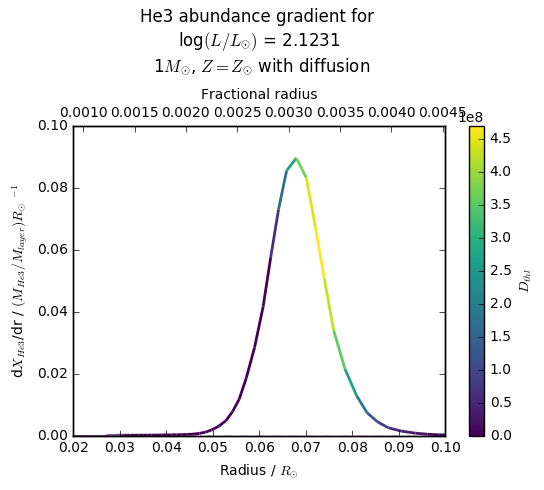
\includegraphics[scale=0.6]{../mu_test_data/mu_test_graphs/eq_logL=2p1231_He3_radius_gradient_Dthl_color.png}
\caption{$^{3}$He abundance gradient for model with $Z = Z_{\sun}$, $M = 1M_{\sun}$ and diffusion effects included, at a point $\log(L/L_{\sun}) = 2.1231$}
\label{dHe3/dr_colour}
\end{center}
\end{figure}

\begin{figure}
\begin{center}
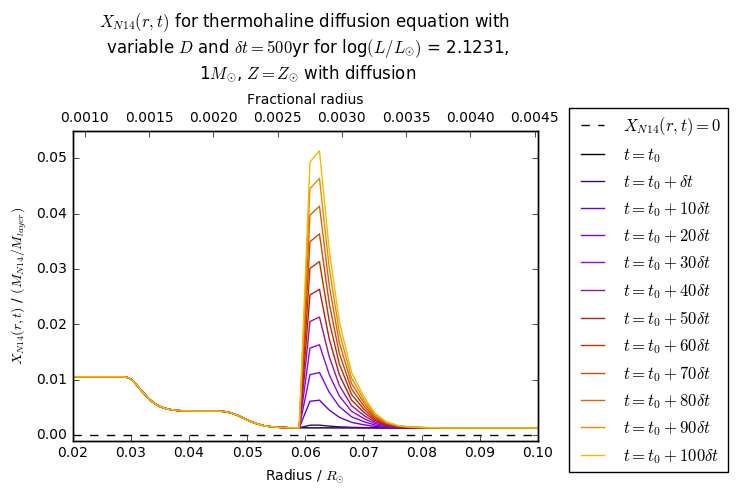
\includegraphics[scale=0.4]{../mu_test_data/mu_test_graphs/eq_logL=2p1231_time_diff_eq_Dvar_10dt_dmu_k_lim.png}
\caption{$^{14}$N abundance time derivative for model with $Z = Z_{\sun}$, $M = 1M_{\sun}$ and diffusion effects included, at a point $\log(L/L_{\sun}) = 2.1231$}
\label{dXN14/dt_colour}
\end{center}
\end{figure}

\subsection{Differential extinction}
Initially, ****the values of $A_{X}/A_{V}$ were fitted using a simple function of $T_{\textnormal{eff}}$ only, containing 3 free parameters, denoted by $a$,$b$ and $c$. The results of this stage are stored in the function $A_{1} = A_{X}/A_{V}(T_{\textnormal{eff}})$. $A_{1}$ took on one of two function forms, depending on the relative performance of both in each filter. The first case, referred to in Table \ref{R1_coeffs_table} by the abbreviation `pow', models a fit of the following power-law form:

\begin{equation}
A_{1,\textnormal{pow}} (T_{\textnormal{eff}}) = a (T_{\textnormal{eff}})^{b} + c
\label{Teff_pow}
\end{equation}

while the second case (denoted by `exp') models an exponential:

\begin{equation}
A_{1,\textnormal{exp}} (T_{\textnormal{eff}}) = a \exp{(b T_{\textnormal{eff}})} + c
\label{Teff_exp}
\end{equation}

This first fitting step was carried out with ****no anchor points, for  fixed values of stellar surface gravity (log($g$/cm s$^{-1}$) = 5.0) and metallicity ($Z = Z_{\sun}$). Due to a low-$T_{\textnormal{eff}}$ artefact present in the data for several filters in both the WFC3 and Gaia systems, this project only analysed data for $T_{\textnormal{eff}} \geq 4500$K.

\begin{table}
\begin{tabular}{ccccccccc}
\hline
\multirow{2}{*}{System} & \multirow{2}{*}{Filter} & \multirow{2}{*}{$A_{1}$ function} & \multicolumn{6}{c}{$A_{1}$ coefficients} \\ \cline{4-9} % & \multicolumn{3}{c}{$A_{2}$ coefficients} \\ \cline{2-7}
%\textbf{Filter} & \textbf{AUC value for FRB data} \\
& & & $a$ & $\sigma_{a}$ & $b$ & $\sigma_{b}$ & $c$ & $\sigma_{c}$ \\ \hline
& f218w & exp & cell1 & cell2 & cell3 & cell1 & cell2 & cell3 \\
& f225w & exp & cell4 & cell5 & cell6 & cell1 & cell2 & cell3 \\
& f275w & exp & cell7 & cell8 & cell9 & cell1 & cell2 & cell3 \\
& f300x & pow & cell7 & cell8 & cell9 & cell1 & cell2 & cell3 \\
& f336w & pow & cell7 & cell8 & cell9 & cell1 & cell2 & cell3 \\
& f390w & pow & cell7 & cell8 & cell9 & cell1 & cell2 & cell3 \\
WFC3 & f438w & pow & cell7 & cell8 & cell9 & cell1 & cell2 & cell3 \\
& f475w & pow & cell7 & cell8 & cell9 & cell1 & cell2 & cell3 \\
& f555w & pow & cell7 & cell8 & cell9 & cell1 & cell2 & cell3 \\
& f606w & pow & cell7 & cell8 & cell9 & cell1 & cell2 & cell3 \\
& f625w & pow & cell7 & cell8 & cell9 & cell1 & cell2 & cell3 \\
& f775w & pow & cell7 & cell8 & cell9 & cell1 & cell2 & cell3 \\
& f814w & pow & cell7 & cell8 & cell9 & cell1 & cell2 & cell3 \\ \hline
& G & pow & cell7 & cell8 & cell9 & cell1 & cell2 & cell3 \\
Gaia & G\textsubscript{bp} & pow & cell7 & cell8 & cell9 & cell7 & cell8 & cell9 \\
& G\textsubscript{rp} & pow & cell7 & cell8 & cell9 & cell7 & cell8 & cell9 \\

\end{tabular}
\label{R1_coeffs_table}
\end{table}

As shown in Figure****, for some filters, there are significant changes in the extinction ratio values at fixed $T_{\textnormal{eff}}$ ($|\delta A| > 0.02$), due to changes in log($g$), $Z$ or both.

\begin{figure}
\begin{center}
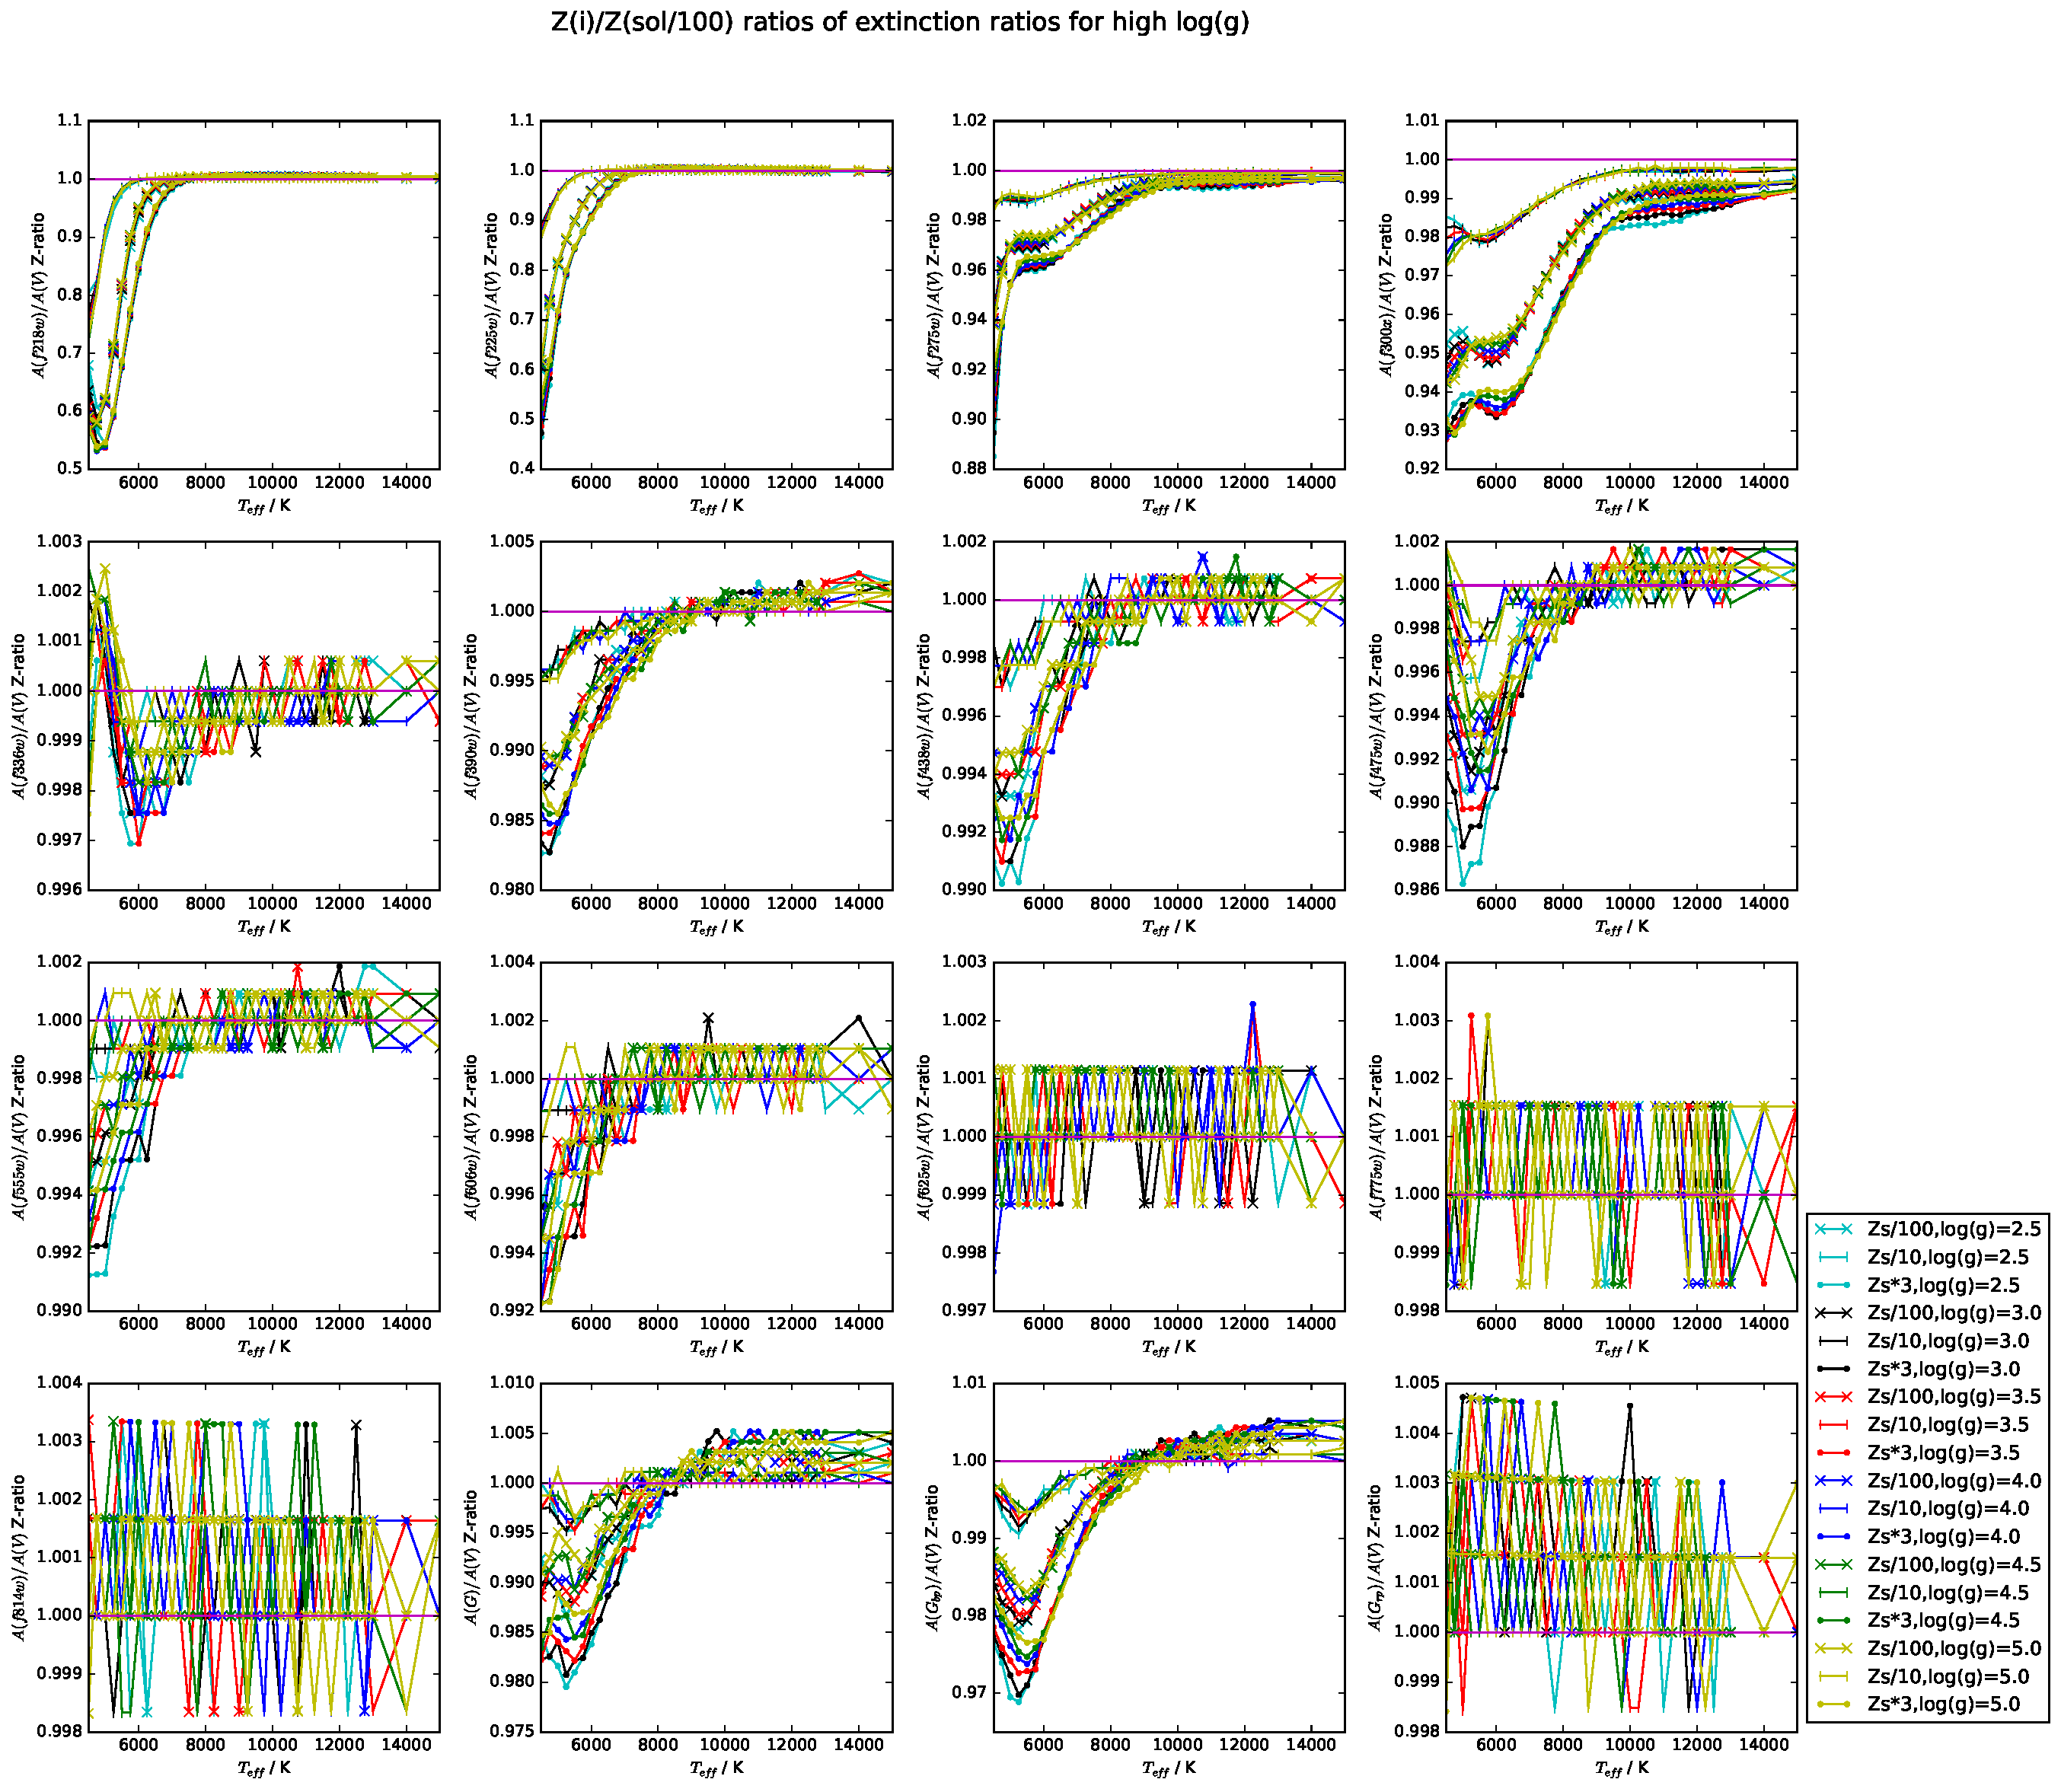
\includegraphics[scale=0.3]{../Aall_ratio_Zs_div_Z2_effect_high_logg_zoom_15000.pdf}
\caption{****psrsoft image output for a simulated pulsar data file}
\label{all_Z_Z2_ratio}
\end{center}
\end{figure}

\begin{figure}
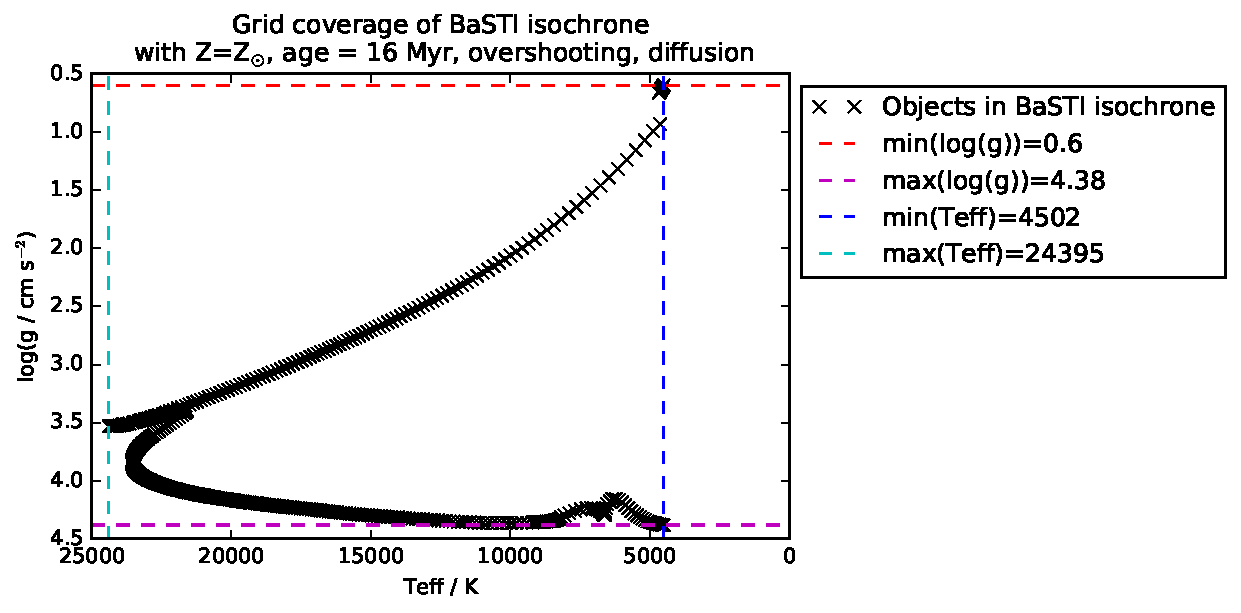
\includegraphics[scale=0.4]{../wfc3_16_23Myr_10Gyr_complex_solar/wfc3_ATLAS9_grid_BaSTI_coverage_c16_complex_Zsol_4500.pdf}
\caption{$T_{\textnormal{eff}}$-log($g$) grid coverage by a 16 Myr, $Z_{\sun}$ BaSTI isochrone ****including mass-loss, core overshooting and }
\label{BaSTI_coverage}
\end{figure}

% ****FORMAT FOR INCLUDING PDF IMAGES!!!
% for guidance, see phd_work/grfguide.pdf
%\includegraphics[<options>]{filename.pdf}



\citet{2004astro.ph..5087C}


\section{Discussion}
\subsection{Thermohaline mixing}
As shown in Figure \ref{dXN14/dt_colour}, the conditions for thermohaline mixing are reproduced in the BaSTI code. The location of the regions for which these conditions apply is located in the upper, and therefore cooler, layers of the hydrogen fusion shell,

So far, by measuring abundances of species which both are hydrogen fusion products and are not involved in $^3$He burning, such as $^{14}$N, it has been established that the existing BaSTI stellar evolution model creates the conditions for thermohaline mixing to occur in the radiative zone of a low-mass, post-FDU RGB star. It has also been shown that, as expected, the conditions are created by molecular weight inversions arising from $^{3}$He burning.

While the physical process and impacts of thermohaline mixing have been successfully implemented in other stellar evolution codes, such as MESA and STAREVOL, BaSTI has not yet been modified to include these in the iterative calculations. Achieving this is a significant goal because, as demonstrated by \citet{2015MNRAS.446.2673L} in the particular case of lithium abundances, there can be significant differences in predictions of abundances between different stellar evolution codes. Adding BaSTI to the list of codes available for future comparative studies would provide more scope to study potential sources of error, such as the model time-step and $C_{thl}$ value effects on abundances noted by \citet{2015MNRAS.446.2673L}. Of particular interest is the $C_{thl}$ free-parameter value, as there are many proposed values, from authors using different approaches and models, which differ in some cases by at least an order of magnitude.

**** modelling/integrating other effects into BaSTI



\subsection{Differential extinction}

\section{Future work}

This work, although confirming feasibility of thermohaline mixing in BaSTI, has yet to implement the effects of the resultant chemical mixing on the models of the star at times following the initial mixing.

Isochrones****

\bibliographystyle{mnras} % unsrtnat
\bibliography{transfer_report}

\end{document}